\documentclass[10pt]{article}

\usepackage[a4paper,margin=1.9cm]{geometry}
\usepackage{amsmath,amssymb}
\usepackage{booktabs}
\usepackage{graphicx}
\usepackage{microtype}
\usepackage{tabularx}
\usepackage{array}
\usepackage{enumitem}
\usepackage{xcolor}
\usepackage{caption}
\usepackage{natbib}
\usepackage[hidelinks]{hyperref}

\definecolor{accent}{HTML}{1F6F8B}
\definecolor{softgray}{HTML}{F2F4F5}
\hypersetup{
  colorlinks=true,
  linkcolor=accent,
  citecolor=accent,
  urlcolor=accent
}

\captionsetup{font=small,labelfont=bf}
\setlist[itemize]{leftmargin=1.5em,itemsep=2pt,topsep=3pt}
\setlength{\parindent}{1.2em}
\setlength{\parskip}{0.15em}
\setlength{\tabcolsep}{5pt}
\renewcommand{\arraystretch}{1.12}
\newcolumntype{Y}{>{\raggedright\arraybackslash}X}

\title{\textbf{From Behavior Cloning to Dataset Aggregation:}\\
An Empirical Study of Distribution Shift in Imitation Learning}
\author{Huilin Luo}
\date{}

\begin{document}
\maketitle

\begin{abstract}
Imitation learning trains a policy from expert state--action examples, but a
policy that is accurate on recorded demonstrations can still fail after its own
small mistakes move it into unfamiliar states. This paper explains that gap from
first principles and tests it in four connected experiments. First, an archived
convolutional behavior-cloning model maps road images to steering angles and
reaches a validation mean squared error (MSE) of 0.0144 on 7,698 driving records.
Second, a controlled CartPole experiment compares behavior cloning (BC) with
Dataset Aggregation (DAgger). Under a deliberately wider test-state
distribution, BC obtains a mean return of 309.35 and a 20\% success rate, whereas
DAgger reaches a return of 500 and 100\% success after one aggregation round.
Independent state-distribution analysis shows that DAgger reduces pooled action
error from 25.08\% to 0.93\% and expands the demonstrated cart-position range by
13.96 times. Finally, BC, BC-RNN, and BC-Transformer are compared on official
RoboMimic low-dimensional demonstrations for Lift, Can, Square, and Transport.
The Transformer has the lowest offline action MSE on all four tasks and reduces
the four-task mean by 15.53\% relative to feed-forward BC. The results support a
specific conclusion: matching the policy's deployment distribution is at least
as important as reducing training loss. They also show why offline action MSE
must not be reported as closed-loop task success.
\end{abstract}

\section{Introduction}

Imitation learning (IL) asks a learner to act like an expert without first
discovering a reward function or exploring every consequence of a bad action.
The idea has a long history in autonomous driving, from ALVINN's direct mapping
from sensors to steering direction \citep{pomerleau1989alvinn} to modern
convolutional image-to-control systems \citep{bojarski2016end}. It is also
attractive for robot manipulation, where human demonstrations can be easier to
collect than a reward function that reliably distinguishes every failure mode
\citep{mandlekar2022robomimic}.

The simplest IL method, behavior cloning (BC), treats each expert state--action
pair as an ordinary supervised-learning example. This is easy to implement, but
the ordinary independent and identically distributed assumption is broken at
deployment: a policy's action changes the next state, so its future inputs
depend on its earlier predictions. A small error can therefore create a state
that the expert dataset never covered, causing a second, larger error. This
feedback mechanism is called covariate shift or compounding error. DAgger
addresses it by repeatedly visiting states with the current policy, asking the
expert what should have been done there, and adding those labeled states to the
training set \citep{ross2011dagger}.

This paper studies that mechanism rather than merely listing IL algorithms. Its
contributions are:
\begin{itemize}
  \item a beginner-oriented derivation connecting maximum likelihood, MSE, and
  cross-entropy behavior-cloning losses;
  \item a step-by-step explanation of why an expert-distribution error rate can
  lead to a quadratic-in-horizon failure bound, and why DAgger removes the extra
  horizon factor in the corresponding simplified argument;
  \item a controlled CartPole study linking data aggregation to state coverage,
  action error, return, and success rate; and
  \item a four-task RoboMimic comparison that separates offline action
  prediction from closed-loop robot success.
\end{itemize}

\section{Background}

\subsection{Sequential Decisions and Demonstrations}

Consider a finite-horizon decision process
\[
  \mathcal{M}=(\mathcal{S},\mathcal{A},P,\rho_0,T).
\]
Here, $\mathcal{S}$ is the state space, $\mathcal{A}$ is the action space,
$P(s_{t+1}\mid s_t,a_t)$ is the transition probability, $\rho_0$ is the
initial-state distribution, and $T$ is the maximum number of steps. A policy
$\pi(a\mid s)$ specifies how an action is selected in a state. The expert policy
is $\pi_E$ and the learned policy, parameterized by weights $\theta$, is
$\pi_\theta$.

A rollout produces a trajectory
\[
  \tau=(s_1,a_1,s_2,a_2,\ldots,s_T,a_T).
\]
The notation $d_\pi^t(s)$ means the probability of visiting state $s$ at time
$t$ when actions are chosen by $\pi$. This distribution is essential: even when
two policies start from the same $\rho_0$, different actions generally produce
different later state distributions. Expert demonstrations form the dataset
\[
  \mathcal{D}_E=\{(s_i,a_i)\}_{i=1}^{N},
\]
where $N$ is the number of labeled state--action pairs. IL learns a policy from
$\mathcal{D}_E$ rather than from an explicitly supplied reward.

\subsection{Behavior Cloning as Maximum Likelihood}

Behavior cloning fits $\pi_\theta$ by empirical risk minimization:
\begin{equation}
  \theta^\star
  =\arg\min_\theta \frac{1}{N}
  \sum_{i=1}^{N}
  \ell\!\left(\pi_\theta(s_i),a_i\right).
  \label{eq:bc-objective}
\end{equation}
In Eq.~\eqref{eq:bc-objective}, $\theta^\star$ is the fitted parameter vector,
$\ell$ is a per-example loss, $s_i$ is an expert-observed state, and $a_i$ is
the expert action.

For a discrete action set, the network outputs class probabilities. Maximum
likelihood gives the cross-entropy loss
\begin{equation}
  \mathcal{L}_{\mathrm{CE}}(\theta)
  =-\frac{1}{N}\sum_{i=1}^{N}
  \sum_{k=1}^{K}y_{ik}\log \pi_\theta(a=k\mid s_i),
  \label{eq:ce}
\end{equation}
where $K$ is the number of actions and $y_{ik}=1$ only when expert example $i$
uses action $k$. Minimizing Eq.~\eqref{eq:ce} increases the probability assigned
to the expert's action.

For continuous controls, suppose that an expert action is a noisy observation
around the policy output:
\[
  p(a_i\mid s_i,\theta)
  =\mathcal{N}\!\left(a_i;\pi_\theta(s_i),\sigma^2 I\right).
\]
The symbols $\mathcal{N}$, $\sigma^2$, and $I$ denote a Gaussian density, a
fixed action-noise variance, and the identity matrix. Taking the negative log
likelihood and dropping terms independent of $\theta$ gives
\begin{align}
  -\frac{1}{N}\sum_{i=1}^{N}\log p(a_i\mid s_i,\theta)
  &=
  \frac{1}{2\sigma^2N}
  \sum_{i=1}^{N}
  \left\|a_i-\pi_\theta(s_i)\right\|_2^2+C.
  \label{eq:mse-derivation}
\end{align}
Because $1/(2\sigma^2)$ and $C$ are constant, maximum likelihood is equivalent
to minimizing MSE. This is why both the steering-angle model and the continuous
RoboMimic policies use squared action error.

\subsection{Why Small BC Errors Can Compound}

Assume that BC makes a one-step error with probability at most $\epsilon$ on
states distributed like the expert demonstrations. At time $t$, the learner may
still be on the expert-like path, or it may have left that path because of an
earlier error. A union bound gives
\[
  \Pr(\text{an earlier error before }t)\leq (t-1)\epsilon.
\]
In a worst-case argument, the policy can be completely unreliable after leaving
the demonstrated distribution. Its error probability at time $t$ is then
bounded by
\[
  \Pr(\text{error at }t)
  \leq \epsilon+(t-1)\epsilon=t\epsilon.
\]
Summing over the horizon yields
\begin{equation}
  \mathbb{E}[\text{number of errors}]
  \leq \sum_{t=1}^{T}t\epsilon
  =\frac{T(T+1)}{2}\epsilon
  =O(T^2\epsilon).
  \label{eq:quadratic}
\end{equation}
Equation~\eqref{eq:quadratic} is deliberately conservative, but it explains the
failure mechanism to a new reader: supervised accuracy is measured under
$d_{\pi_E}$, while deployment inputs come from $d_{\pi_\theta}$. The original
DAgger analysis formalizes this mismatch through a reduction to no-regret online
learning \citep{ross2011dagger}.

\subsection{DAgger: Label the States the Learner Visits}

At DAgger iteration $j$, data are collected with a mixture of the expert and the
current learner:
\begin{equation}
  \pi_j^{\mathrm{mix}}
  =\beta_j\pi_E+(1-\beta_j)\pi_j,
  \qquad \beta_j=\lambda^j.
  \label{eq:mixture}
\end{equation}
Equation~\eqref{eq:mixture} means that the expert action is executed with
probability $\beta_j$ and the learner action with probability $1-\beta_j$.
$\lambda\in[0,1]$ is the decay factor, $j$ is the iteration number, and
$\pi_j$ is the policy before retraining. Regardless of which action is executed,
the expert labels every visited state. The aggregated dataset is
\begin{equation}
  \mathcal{D}_{j}
  =\mathcal{D}_{j-1}\cup
  \{(s,\pi_E(s)):s\sim d_{\pi_j^{\mathrm{mix}}}\},
  \qquad
  \pi_{j+1}=\operatorname{Train}(\mathcal{D}_{j}).
  \label{eq:dagger}
\end{equation}
Here, $s\sim d_{\pi_j^{\mathrm{mix}}}$ indicates a state visited by the mixed
rollout policy. If retraining achieves average error $\epsilon_D$ under the
learner-relevant aggregated distribution, then the analogous sum is
$\sum_{t=1}^{T}\epsilon_D=T\epsilon_D$, rather than the quadratic expression in
Eq.~\eqref{eq:quadratic}. The full guarantee requires no-regret assumptions, but
the simplified calculation captures the central idea: DAgger trains on the
inputs that its policy will actually encounter.

\subsection{Function Approximators for Imitation Policies}

For images, a convolutional layer computes local visual features:
\begin{equation}
  h_{i,j,k}
  =\phi\!\left(
  b_k+\sum_{c=1}^{C}\sum_{u=1}^{U}\sum_{v=1}^{V}
  W_{u,v,c,k}X_{i+u,j+v,c}\right).
  \label{eq:conv}
\end{equation}
$X$ is the input image, $W$ is a learned $U\times V$ filter bank, $c$ indexes
input channels, $k$ indexes output features, $b_k$ is a bias, and $\phi$ is an
activation such as ReLU. Weight sharing lets the same road feature be detected
at many image locations with far fewer parameters than a fully connected layer.

For temporal robot observations, the experiment compares an LSTM and a
Transformer. Given an encoded observation $x_t$, an LSTM updates
\begin{align}
  i_t&=\sigma(W_ix_t+U_ih_{t-1}+b_i),&
  f_t&=\sigma(W_fx_t+U_fh_{t-1}+b_f),\nonumber\\
  o_t&=\sigma(W_ox_t+U_oh_{t-1}+b_o),&
  g_t&=\tanh(W_gx_t+U_gh_{t-1}+b_g),\nonumber\\
  c_t&=f_t\odot c_{t-1}+i_t\odot g_t,&
  h_t&=o_t\odot\tanh(c_t).
  \label{eq:lstm}
\end{align}
The vectors $i_t,f_t,o_t$ are input, forget, and output gates; $g_t$ is a
candidate update; $c_t$ is memory; $h_t$ is the hidden state; $W_\cdot$ and
$U_\cdot$ are learned matrices; and $\odot$ is elementwise multiplication. The
gates provide paths through which information and gradients can persist
\citep{hochreiter1997lstm}.

A Transformer instead compares all positions in a short context through scaled
dot-product attention \citep{vaswani2017attention}:
\begin{equation}
  Q=XW_Q,\quad K=XW_K,\quad V=XW_V,\qquad
  \operatorname{Attn}(Q,K,V)
  =\operatorname{softmax}\!\left(\frac{QK^\top}{\sqrt{d_k}}\right)V.
  \label{eq:attention}
\end{equation}
$X\in\mathbb{R}^{H\times d}$ contains $H$ encoded observations of width $d$;
$Q$, $K$, and $V$ are queries, keys, and values; $W_Q,W_K,W_V$ are learned
projections; and $d_k$ is the key width. Each row of the softmax is a set of
weights over time. Dividing by $\sqrt{d_k}$ prevents dot products from growing
too large as the representation width increases. Multiple heads repeat this
operation with different projections, allowing different temporal relations to
be represented.

\section{Method}

\subsection{Study Design}

The experiments progress from an archived perception policy to a controlled
distribution-shift test and then to official robot demonstrations. Table
\ref{tab:study-design} summarizes their roles. Experiment 3 is an analysis layer:
it reads machine-generated outputs from the other experiments and quantifies the
mechanism behind the performance change.

\begin{table}[ht]
  \centering
  \caption{Connected experimental design.}
  \label{tab:study-design}
  \small
  \begin{tabularx}{\textwidth}{@{}>{\raggedright\arraybackslash}p{1.2cm}>{\raggedright\arraybackslash}p{2.6cm}Y Y@{}}
    \toprule
    Exp. & Domain & Main comparison & Evidence \\
    \midrule
    1 & Image steering & CNN behavior cloning & Train/validation MSE and retained model \\
    2 & CartPole & Fixed BC vs.\ DAgger & Return, success, beta ablation, action error \\
    3 & Cross-experiment analysis & Expert, BC, and DAgger state distributions & Percentile coverage and policy-visited states \\
    4 & Robot manipulation & BC, BC-RNN, BC-Transformer & Official-data validation MSE and trajectory bootstrap intervals \\
    \bottomrule
  \end{tabularx}
\end{table}

\subsection{Experiment 1: Visual Behavior Cloning}

The driving dataset contains 7,698 records. Each record supplies center, left,
and right camera paths plus a steering angle. A fixed seed of 42 produces 6,158
training and 1,540 validation records. Training randomly selects a camera,
applies steering corrections $(+0.25,0,-0.25)$, introduces shadows and crop
variation, flips half of each batch, and resizes images to
$32\times128\times3$. Validation uses only the center camera and deterministic
cropping.

The CNN has three convolution--pooling blocks with 16, 32, and 64 filters,
followed by dense layers of sizes 500, 100, 20, and 1. Dropout rates are 0.5 and
0.25. The 972,225 parameters are optimized for 30 epochs with Adam at learning
rate $10^{-4}$ and batch size 128. The raw simulator images are no longer in the
repository; therefore this study verifies the retained source, model hash, and
loss artifact rather than claiming a new end-to-end retraining run.

\subsection{Experiments 2--3: Controlled CartPole Shift}

The CartPole state is
\[
  s=[x,\dot{x},\theta,\dot{\theta}],
\]
where $x$ is cart position and $\theta$ is pole angle. Actions 0 and 1 apply a
left or right force. The local environment matches the standard CartPole
constants and Euler update used by Gymnasium \citep{towers2024gymnasium}: the
episode ends at $|x|>2.4$ m, $|\theta|>12^\circ$, or 500 steps.

The deterministic expert uses the stabilizing score
\begin{equation}
  z(s)=1.05\theta+0.19\dot{\theta}+0.012x+0.018\dot{x}
  +0.35\theta^3+b(x),
  \quad
  \pi_E(s)=\mathbb{1}[z(s)>0],
  \label{eq:expert}
\end{equation}
where $b(x)=0.055\,\operatorname{sign}(x)$ when $|x|>1.65$ and zero otherwise.
$\mathbb{1}[\cdot]$ is one when its condition is true. Initial BC data comprise
two 500-step expert rollouts from the narrow reset interval $[-0.02,0.02]^4$.
Evaluation and DAgger collection use the wider intervals
$x\in[-0.35,0.35]$, $\dot{x}\in[-0.45,0.45]$,
$\theta\in[-0.105,0.105]$, and
$\dot{\theta}\in[-0.45,0.45]$.

Both BC and DAgger use a standardized MLP with two 32-unit tanh layers. The main
DAgger run uses six iterations, ten rollouts per iteration, and
$\beta_j=0.5^j$. Beta ablations use $\lambda\in\{0.9,0.5,0.1\}$ with three
rollouts per iteration. Every policy is evaluated on the same 80 fixed seeds,
and an episode of at least 475 steps is counted as successful.

To measure more than return, 40 independent seeds generate states visited by
the expert, BC, and DAgger policies. For a policy probability
$p_\theta(s)=\Pr_\theta(a=1\mid s)$ and deterministic expert label $y(s)$, the
action-probability error is
\begin{equation}
  \operatorname{MSE}_a
  =\frac{1}{M}\sum_{m=1}^{M}
  \left(p_\theta(s_m)-y(s_m)\right)^2,
  \label{eq:action-mse}
\end{equation}
where $M$ is the number of independently collected states. State coverage for
each coordinate is the 99th percentile minus the 1st percentile; this robust
span is less sensitive to isolated extreme points than a raw minimum--maximum
range.

\subsection{Experiment 4: Official RoboMimic Offline Benchmark}

The robot benchmark uses official RoboMimic v1.5 proficient-human
low-dimensional HDF5 data \citep{mandlekar2022robomimic}. Each task has 200
demonstration trajectories and uses the official 180/20 train/validation
trajectory masks, preventing adjacent frames from crossing the split.
Observation normalization is computed from training trajectories only.

For context length $H=10$, the policy receives
$s_{t-H+1:t}$; early windows are padded with their first observation. Feed-forward
BC uses only the last observation and a 256--256 ReLU MLP. BC-RNN projects to
128 dimensions and applies a one-layer 128-unit LSTM. BC-Transformer uses a
128-dimensional embedding, learned positional vectors, two encoder layers, four
attention heads, and a 256-dimensional feed-forward sublayer. Each action head
ends in tanh.

All models minimize the same elementwise validation loss
\begin{equation}
  \mathcal{L}_{\mathrm{robot}}
  =\frac{1}{Nd_a}\sum_{i=1}^{N}
  \sum_{q=1}^{d_a}
  \left(\hat a_{i,q}-a_{i,q}\right)^2,
  \label{eq:robot-mse}
\end{equation}
where $d_a$ is the action dimension, $a_{i,q}$ is expert component $q$, and
$\hat a_{i,q}$ is its prediction. AdamW \citep{loshchilov2019adamw} uses
learning rate $3\times10^{-4}$, weight decay $10^{-4}$, batch size 512, at most
12 epochs, and early-stopping patience 4. Transport is uniformly subsampled to
60,000 train windows; the other tasks use all available train windows.

Uncertainty is summarized by resampling the 20 validation-trajectory MSE values
with replacement 2,000 times. The 2.5th and 97.5th percentiles of the resampled
means form a 95\% bootstrap interval. This interval captures variation among
held-out trajectories, not variation across random training seeds.

\section{Experiments}

\subsection{Reproducibility Scope}

Experiments 2--4 were executed on Windows 11 with Python 3.12.13. CartPole used
fixed seed 20260730, NumPy 2.3.5, and scikit-learn 1.9.0. The robot benchmark
used a deterministic seed family rooted at 20260730 (with fixed model offsets)
and ran with PyTorch 2.12.1 on CPU and h5py 3.15.1. Experiment 1 was trained previously
with TensorFlow 2.15.0; its retained \texttt{model.h5} has SHA-256
\texttt{9a9008c5...f3c61ba9}. No simulator success rate is available for that
archived experiment.

\subsection{Experiment 1: An Offline Fit Is Not a Driving Guarantee}

The final training MSE is 0.0684 and validation MSE is 0.0144. The lower
validation value should not be read as evidence that validation is ``easier to
overfit.'' Training batches contain stronger random augmentation and use dropout,
while validation is deterministic and dropout-free, so the two losses are not
measured under identical input conditions. Figure~\ref{fig:driving-loss} shows
that the image-to-steering regression converged, but it cannot establish stable
closed-loop driving without simulator rollouts.

\begin{figure}[ht]
  \centering
  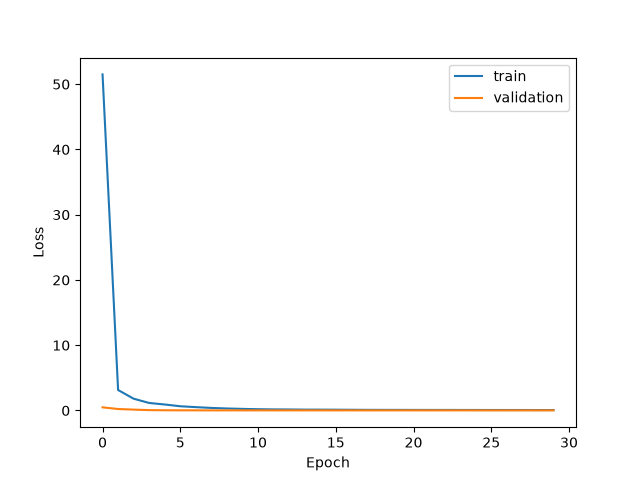
\includegraphics[width=0.68\textwidth]{assets/exp1_loss.png}
  \caption{Archived CNN behavior-cloning loss over 30 epochs. The artifact
  supports offline convergence only; the original image data and a
  machine-readable simulator success rate are unavailable.}
  \label{fig:driving-loss}
\end{figure}

\subsection{Experiment 2: DAgger Repairs the Deliberate Distribution Shift}

Table~\ref{tab:cartpole-main} gives closed-loop results on 80 matched seeds. BC
learns from 1,000 narrow-reset samples and succeeds on only 20\% of the wide
resets. After the first DAgger iteration, the policy reaches the 500-step limit
on every evaluation seed and remains there through iteration 6. The final
dataset contains 30,701 samples, so the improvement combines better
distributional coverage with a 30.70-fold increase in labeled data.

\begin{table}[ht]
  \centering
  \caption{CartPole closed-loop evaluation on 80 shared seeds.}
  \label{tab:cartpole-main}
  \small
  \begin{tabular}{@{}lrrrrr@{}}
    \toprule
    Policy & Samples & Mean return & Std. & Median & Success \\
    \midrule
    BC & 1,000 & 309.35 & 123.63 & 276 & 20\% \\
    DAgger, iter.\ 1 & 5,701 & 500.00 & 0.00 & 500 & 100\% \\
    DAgger, iter.\ 6 & 30,701 & 500.00 & 0.00 & 500 & 100\% \\
    Expert & -- & 500.00 & 0.00 & 500 & 100\% \\
    \bottomrule
  \end{tabular}
\end{table}

\begin{figure}[ht]
  \centering
  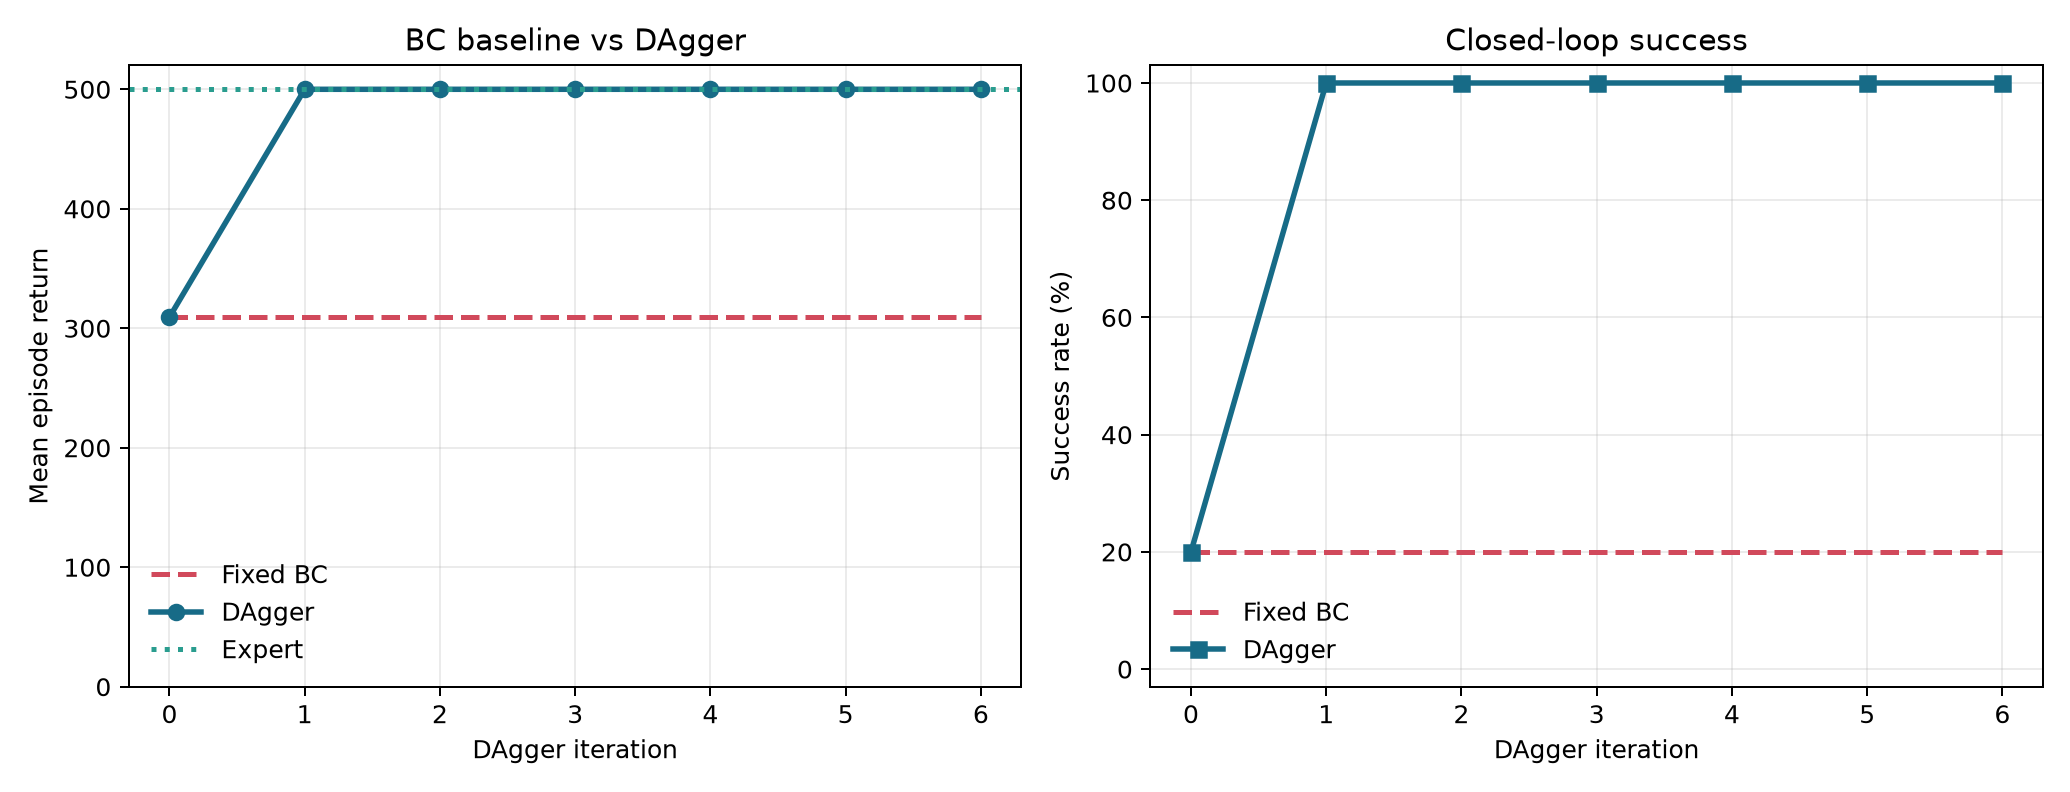
\includegraphics[width=\textwidth]{assets/exp2_learning_curve.png}
  \caption{Fixed BC versus DAgger. One round of labeling states reached under
  the wide reset distribution is sufficient to saturate this deterministic
  CartPole setup.}
  \label{fig:dagger-curve}
\end{figure}

The beta ablation does not distinguish decay schedules: $\lambda=0.9$, 0.5, and
0.1 all reach a final mean return of 500 and 100\% success. Their final dataset
sizes are 10,000, 9,393, and 9,707, respectively. Because all three settings
saturate after one iteration, the correct conclusion is not that the schedule is
irrelevant in general; it is that the present task and query budget are too easy
to expose a schedule effect.

\subsection{Experiment 3: Mechanism Analysis}

The pooled independent-state results in Table~\ref{tab:action-error} directly
test whether the improved return corresponds to better expert-action prediction
where policies actually go. DAgger reduces probability MSE by 97.11\%, action
error by 24.15 percentage points, and binary cross-entropy by 98.47\%.

\begin{table}[ht]
  \centering
  \caption{Expert-action prediction on 30,000 pooled policy-visited states.}
  \label{tab:action-error}
  \small
  \begin{tabular}{@{}lrrr@{}}
    \toprule
    Policy & Probability MSE & Action error & Binary CE \\
    \midrule
    BC & 0.221315 & 25.077\% & 1.358322 \\
    DAgger & 0.006405 & 0.927\% & 0.020764 \\
    \bottomrule
  \end{tabular}
\end{table}

\begin{figure}[ht]
  \centering
  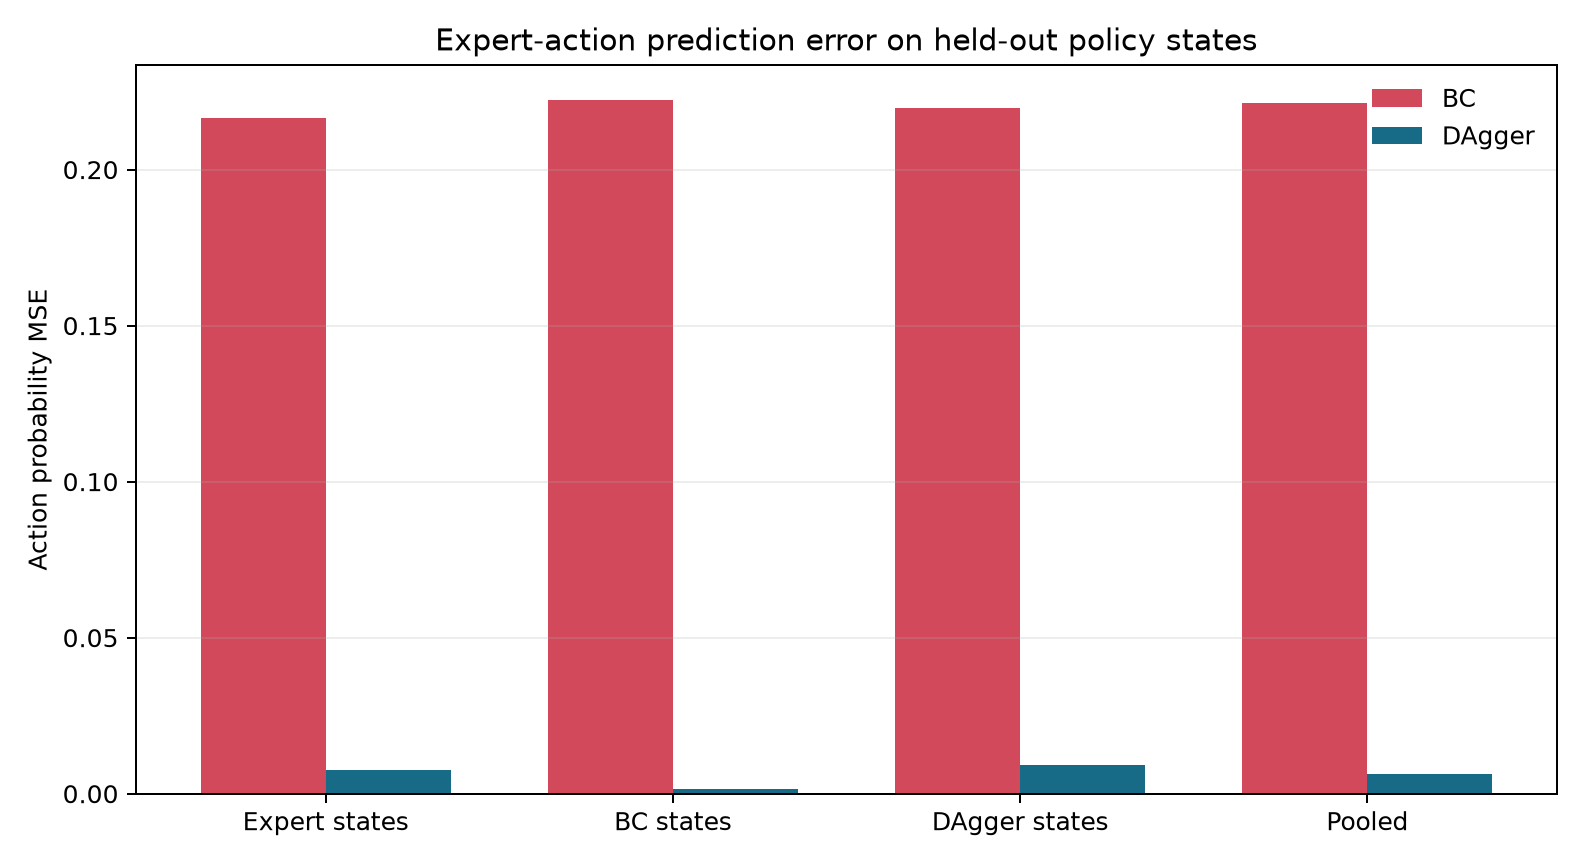
\includegraphics[width=0.94\textwidth]{assets/exp2_action_error.png}
  \caption{Action prediction error on expert-, BC-, DAgger-, and pooled visited
  states. DAgger improves not only its own rollout states but all evaluated
  state groups.}
  \label{fig:action-error}
\end{figure}

The aggregated dataset also broadens the robust state range
(Table~\ref{tab:coverage}). The largest expansion is cart position: the
1st--99th percentile span grows from 0.2731 m to 3.8118 m, or 13.96 times.
Coverage alone does not prove good control, because poor policies can visit many
states. Here it becomes meaningful when combined with lower action error and
higher return.

\begin{table}[ht]
  \centering
  \caption{Robust state coverage before and after DAgger aggregation.}
  \label{tab:coverage}
  \small
  \begin{tabular}{@{}lrrr@{}}
    \toprule
    Coordinate & Initial span & Aggregated span & Gain \\
    \midrule
    Cart position $x$ & 0.2731 & 3.8118 & $13.96\times$ \\
    Cart velocity $\dot{x}$ & 0.4197 & 1.2885 & $3.07\times$ \\
    Pole angle $\theta$ & 0.01476 & 0.09991 & $6.77\times$ \\
    Angular velocity $\dot{\theta}$ & 0.6003 & 0.7906 & $1.32\times$ \\
    \bottomrule
  \end{tabular}
\end{table}

\begin{figure}[ht]
  \centering
  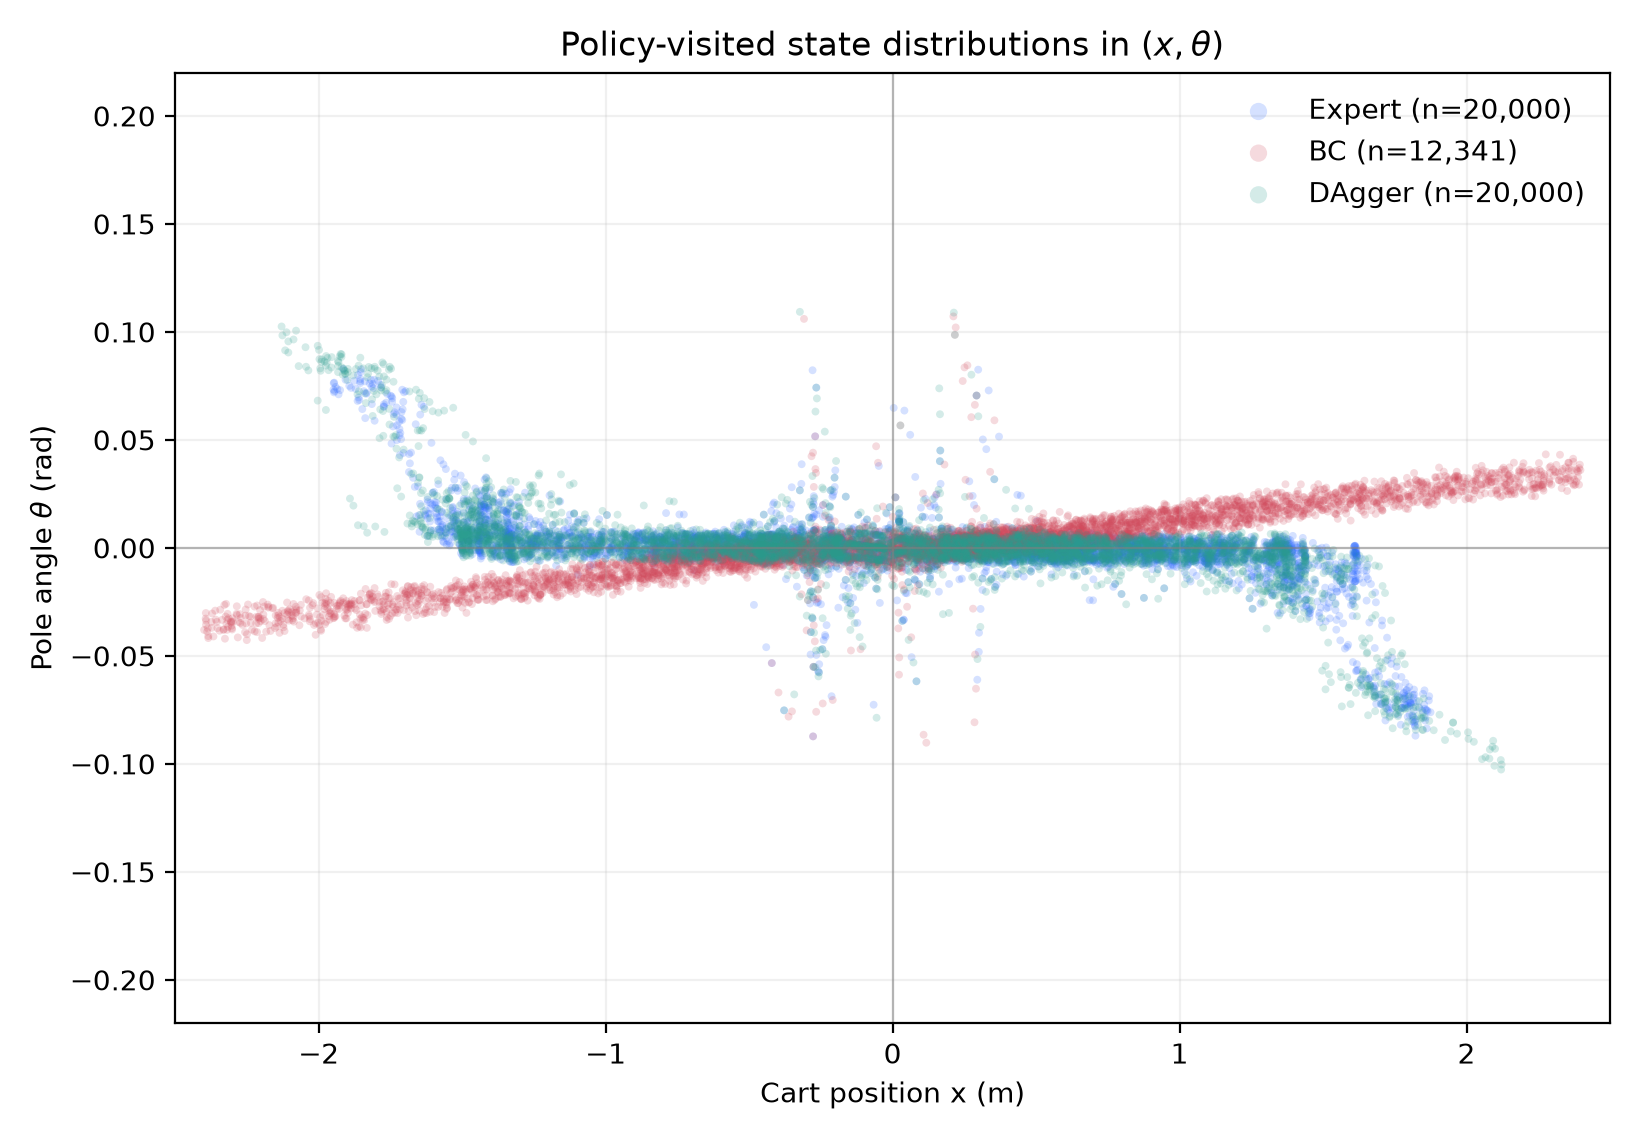
\includegraphics[width=0.88\textwidth]{assets/exp3_policy_state_distribution.png}
  \caption{Policy-visited cart position and pole angle. BC drifts toward the
  $\pm2.4$ m termination boundary, while DAgger more closely follows the expert
  distribution.}
  \label{fig:state-distribution}
\end{figure}

These measurements form a coherent causal chain:
\[
  \begin{aligned}
  \text{learner-state labels}
  &\longrightarrow \text{broader useful coverage}\\
  &\longrightarrow \text{lower on-distribution action error}\\
  &\longrightarrow \text{higher closed-loop return}.
  \end{aligned}
\]
The experiment does not isolate data quantity from data distribution, but the
state plots show why merely fitting the original 1,000 samples is insufficient.

\subsection{Experiment 4: Robot Sequence Models}

Table~\ref{tab:robot-data} describes the official datasets. Lift, Can, and
Square use 7-dimensional single-arm actions; Transport uses 14-dimensional
two-arm actions. Task-level MSE values are comparable across models within a
task, but not necessarily across tasks because their observation and action
dimensions differ.

\begin{table}[ht]
  \centering
  \caption{Official RoboMimic PH low-dimensional datasets.}
  \label{tab:robot-data}
  \small
  \begin{tabular}{@{}lrrrrr@{}}
    \toprule
    Task & Traj. & Samples & Obs. dim. & Act. dim. & Train windows \\
    \midrule
    Lift & 200 & 9,666 & 19 & 7 & 8,640 \\
    Can & 200 & 23,207 & 23 & 7 & 20,883 \\
    Square & 200 & 30,154 & 23 & 7 & 27,165 \\
    Transport & 200 & 93,752 & 59 & 14 & 60,000 \\
    \bottomrule
  \end{tabular}
\end{table}

Table~\ref{tab:robot-results} reports elementwise validation MSE. The Transformer
has the lowest point estimate on every task, reducing MSE relative to BC by
17.15\% on Lift, 12.36\% on Can, 16.53\% on Square, and 16.36\% on Transport.
Across the four task-level point estimates, mean MSE is 0.03154 for BC, 0.03448
for BC-RNN, and 0.02664 for BC-Transformer.

\begin{table}[ht]
  \centering
  \caption{Offline validation action MSE (lower is better).}
  \label{tab:robot-results}
  \small
  \begin{tabular}{@{}lrrrr@{}}
    \toprule
    Model & Lift & Can & Square & Transport \\
    \midrule
    BC & 0.02512 & 0.03294 & 0.03912 & 0.02896 \\
    BC-RNN & 0.02989 & 0.03434 & 0.03980 & 0.03388 \\
    BC-Transformer & \textbf{0.02081} & \textbf{0.02887} &
      \textbf{0.03265} & \textbf{0.02422} \\
    \bottomrule
  \end{tabular}
\end{table}

\begin{center}
  \centering
  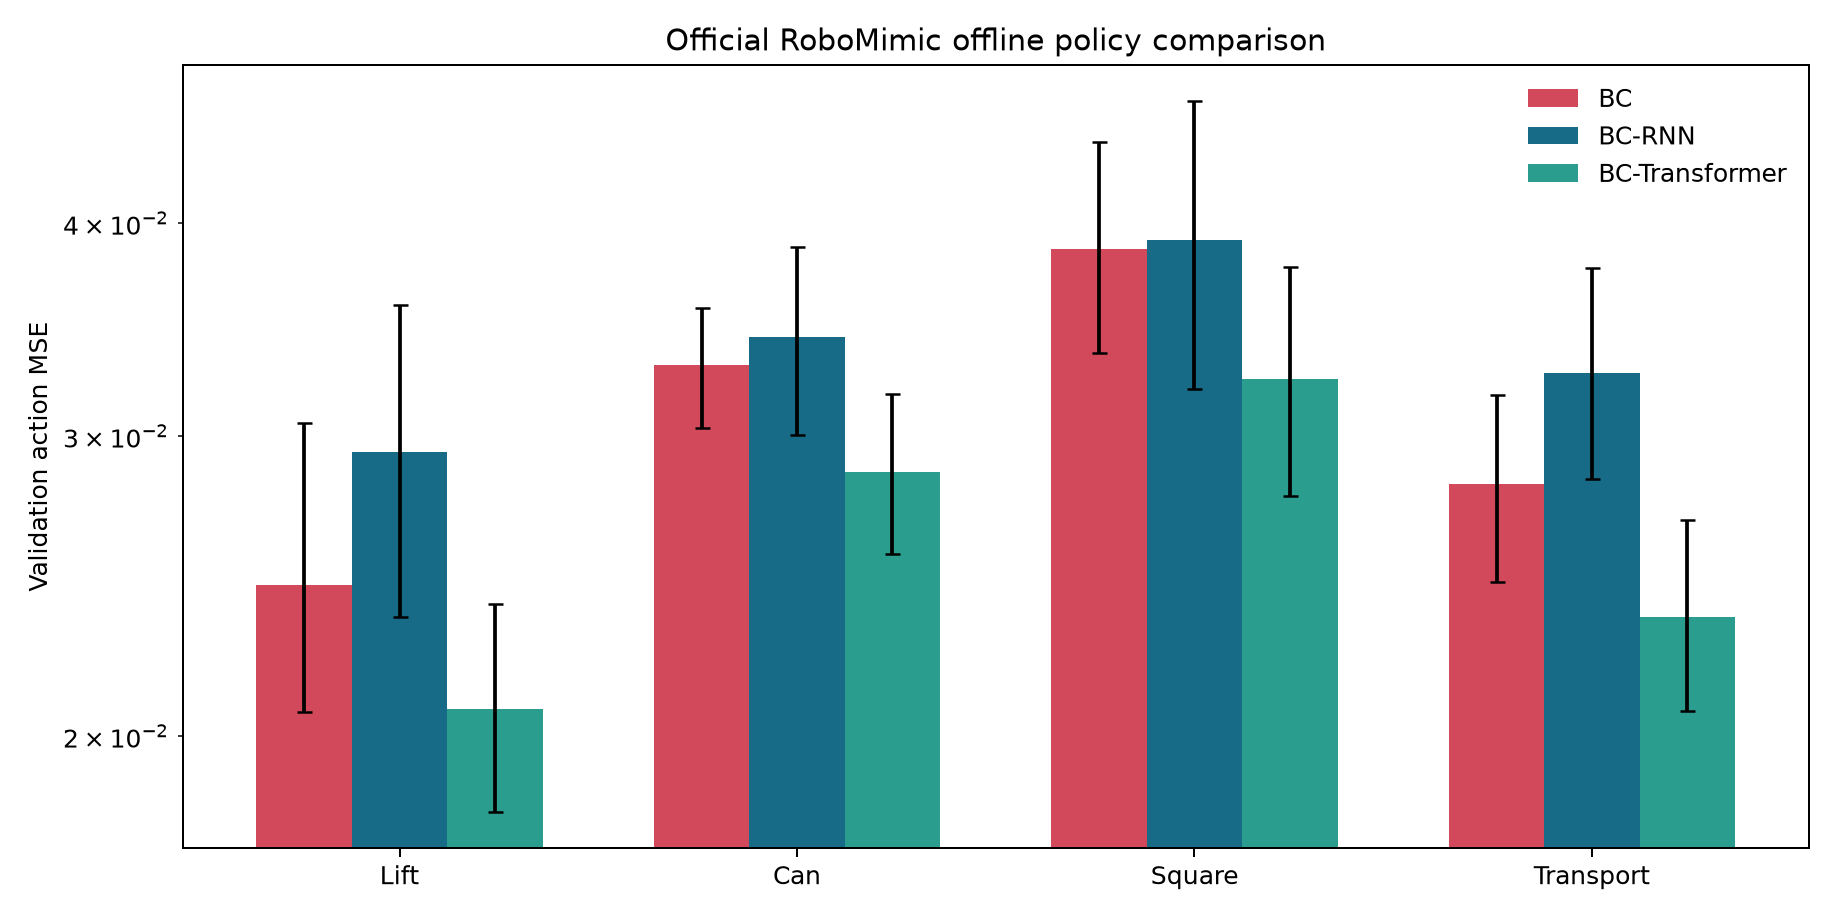
\includegraphics[width=0.94\textwidth]{assets/exp4_official_model_comparison.png}
  \captionsetup{hypcap=false}
  \captionof{figure}{RoboMimic validation action MSE. Error bars are 95\% bootstrap
  intervals over 20 validation trajectories, not confidence intervals over
  repeated model training runs.}
  \label{fig:robot-comparison}
\end{center}

The result is consistent but must be interpreted cautiously. First, the
trajectory bootstrap intervals overlap between models, so a one-seed benchmark
does not establish statistical superiority of the architecture. Second,
BC-Transformer has roughly 286,000--292,000 parameters, compared with
73,000--85,000 for BC, and requires more CPU computation. Third, BC-RNN's weaker
result under a 12-epoch budget shows that adding temporal capacity does not
automatically improve optimization or generalization.

\subsection{Discussion and Limitations}

The CartPole result closely matches the theory: initial BC error is evaluated on
narrow expert states, while failures occur after the policy reaches different
states under wide resets. DAgger queries exactly those states, and both action
error and state distribution move toward the expert. However, the task uses a
deterministic hand-designed expert and dynamics, one training seed, no observation
noise, and a large query budget. The immediate saturation prevents a meaningful
ranking of beta schedules.

The robot study answers a different question. It tests which model predicts held-out
expert actions most accurately under an official trajectory split. It does not
run MuJoCo or robosuite rollouts. Consequently, a validation MSE of 0.02081 on
Lift is not a 97.9\% success rate, nor does lower MSE guarantee fewer compounding
errors. RoboMimic itself emphasizes that offline training objectives and
closed-loop evaluation can select different checkpoints
\citep{mandlekar2022robomimic}.

Finally, the driving experiment has the weakest reproducibility boundary because
the original images are absent. Its source, trained model, and loss curve are
verifiable, but the model cannot be retrained from the delivered repository.
Future work should restore the driving data, run at least three training seeds
for every neural policy, reduce the CartPole query budget to avoid saturation,
and add closed-loop robot success rates using the official simulator stack.

\subsection{Overall Experimental Summary}

Table~\ref{tab:overall-summary} consolidates the four experiments and the
specific claim supported by each one. The distinction between offline
prediction metrics and closed-loop control metrics is retained in the summary.

\begin{table}[ht]
  \centering
  \caption{Overall experimental summary.}
  \label{tab:overall-summary}
  \small
  \begin{tabularx}{\textwidth}{@{}l p{0.28\textwidth} Y@{}}
    \toprule
    Experiment & Method and setting & Main result \\
    \midrule
    Exp.\ 1 & CNN behavior cloning for image-to-steering regression
      & Offline validation MSE: 0.0144. \\
    Exp.\ 2 & DAgger under widened CartPole reset ranges
      & Closed-loop success: 20\% $\rightarrow$ 100\%; mean return:
        309.35 $\rightarrow$ 500.00. \\
    Exp.\ 3 & Policy-state coverage and expert-action error analysis
      & Pooled action error: 25.08\% $\rightarrow$ 0.93\%; cart-position
        coverage: $13.96\times$. \\
    Exp.\ 4 & BC-Transformer on four official RoboMimic tasks
      & Four-task mean offline MSE is 15.53\% lower than feed-forward BC. \\
    \bottomrule
  \end{tabularx}
\end{table}

\section{Conclusion}

Imitation learning is not only supervised learning with actions as labels. The
learner controls the distribution of its future inputs, which makes sequential
prediction fundamentally different from static classification. A simple
union-bound derivation shows how an expert-distribution error $\epsilon$ can
produce an $O(T^2\epsilon)$ worst-case error count, while DAgger's
learner-distribution labeling removes the extra horizon factor in the
corresponding simplified analysis.

The experiments support this explanation. In CartPole, DAgger raises success
from 20\% to 100\%, reduces pooled action error from 25.08\% to 0.93\%, and
expands the demonstrated cart-position range by 13.96 times. On official
RoboMimic data, a compact Transformer lowers four-task mean offline MSE by
15.53\% relative to feed-forward BC, but its confidence intervals, parameter
cost, and lack of closed-loop rollouts prevent a stronger claim. The practical
lesson is precise: report supervised loss, state coverage, and closed-loop
behavior separately, because each measures a different part of an imitation
policy's reliability.

\begingroup
\small
\setlength{\bibsep}{2pt}
\bibliographystyle{plainnat}
\bibliography{references}
\endgroup

\end{document}
